% CVPR 2022 Paper Template
% based on the CVPR template provided by Ming-Ming Cheng (https://github.com/MCG-NKU/CVPR_Template)
% modified and extended by Stefan Roth (stefan.roth@NOSPAMtu-darmstadt.de)

\documentclass[10pt,twocolumn,letterpaper]{article}

%%%%%%%%% PAPER TYPE  - PLEASE UPDATE FOR FINAL VERSION
%\usepackage[review]{cvpr}      % To produce the REVIEW version
\usepackage{cvpr}              % To produce the CAMERA-READY version
%\usepackage[pagenumbers]{cvpr} % To force page numbers, e.g. for an arXiv version

% Include other packages here, before hyperref.
\usepackage{graphicx}
\usepackage{amsmath}
\usepackage{amssymb}
\usepackage{booktabs}
\usepackage{float}
\usepackage{float} % For positionning images
\usepackage{tabularx} % For tables


% It is strongly recommended to use hyperref, especially for the review version.
% hyperref with option pagebackref eases the reviewers' job.
% Please disable hyperref *only* if you encounter grave issues, e.g. with the
% file validation for the camera-ready version.
%
% If you comment hyperref and then uncomment it, you should delete
% ReviewTempalte.aux before re-running LaTeX.
% (Or just hit 'q' on the first LaTeX run, let it finish, and you
%  should be clear).
\usepackage[pagebackref,breaklinks,colorlinks]{hyperref}


% Support for easy cross-referencing
\usepackage[capitalize]{cleveref}
\crefname{section}{Sec.}{Secs.}
\Crefname{section}{Section}{Sections}
\Crefname{table}{Table}{Tables}
\crefname{table}{Tab.}{Tabs.}


%%%%%%%%% PAPER ID  - PLEASE UPDATE
\def\cvprPaperID{****} % *** Enter the CVPR Paper ID here
\def\confName{CVPR}
\def\confYear{2023}

\begin{document}

%%%%%%%%% TITLE - PLEASE UPDATE
\title{Unmasking Sarcasm - Enhancing Sentiment Analysis in E-Commerce Reviews and Questions
}

\author{Hugo Bouy\\
Illinois Tech\\
{\tt\small hbouy@hawk.iit.edu}
% For a paper whose authors are all at the same institution,
% omit the following lines up until the closing ``}''.
% Additional authors and addresses can be added with ``\and'',
% just like the second author.
% To save space, use either the email address or home page, not both
\and
Rémi Kalbe\\
Illinois Tech\\
{\tt\small rkalbe@hawk.iit.edu}
\and
Mathias Roumane\\
Illinois Tech\\
{\tt\small mroumane@hawk.iit.edu}
}
\maketitle

%%%%%%%%% ABSTRACT
% \begin{abstract}
%    The ABSTRACT is to be in fully justified italicized text, at the top of the left-hand column, below the author and affiliation information.
%    Use the word ``Abstract'' as the title, in 12-point Times, boldface type, centered relative to the column, initially capitalized.
%    The abstract is to be in 10-point, single-spaced type.
%    Leave two blank lines after the Abstract, then begin the main text.
%    Look at previous CVPR abstracts to get a feel for style and length.
% \end{abstract}

%%%%%%%%% BODY TEXT
\section{Problem description}
\label{sec:intro}
In an increasingly e-commerce driven world, the analysis of review, comments and questions written by consumers online has become a field of interests.
Understanding opinions and emotions expressed in product feedback/related questions is essential to enhance the user’s experience.
One aspect that might be overlooked in this area is sarcastic and humor detection that can lead to a misinterpretation of these texts.

Humor remains a complex human phenomenon that is far from having a clear definition.
While humor and sarcastic mechanisms are integral to human interaction, its subjective nature makes it a challenging target for computational analysis.
Recent work has been able to open up this area using deep learning and natural language processing advances.
With this project, we will attempt to improve e-commerce review processing using deep learning models for humor disambiguation.

%-------------------------------------------------------------------------

\section{Brief Survey of Previous Work}

Several studies have been conducted over the past years in the ambition of detecting humor and sarcasm:

Jain et al.~\cite{jain2019} delved into the complexities of identifying sarcasm in Amazon reviews. Recognizing sarcasm is crucial for accurate sentiment analysis, especially since sarcastic comments can be misinterpreted by traditional opinion mining methods. They utilized the "Sarcasm Corpus" containing labeled ironic and regular Amazon reviews, extracting features like sentiment scores, punctuation patterns, and contextual elements that consider the contrast between review sentiment and product rating. Their experiments designated the Support Vector Machine (SVM) classifier as the most accurate, emphasizing the role of context in sarcasm detection.

Building upon the idea of sarcasm detection, Poria et al.~\cite{poria2020} introduced a method using deep convolutional neural networks (CNNs). They critiqued traditional methods that treat sarcasm detection as mere text categorization, arguing that such approaches often miss the deeper understanding of language nuances required for sarcasm. Their method integrates sentiment, emotion, and personality features extracted from pre-trained CNNs. By leveraging Twitter data, they contrasted sarcastic sentences with the ground-truth polarity of events. Their experiments with word embeddings from word2vec and a combined CNN-SVM approach demonstrated superior performance on benchmark datasets.

Yaghoobian et al.~\cite{yaghoobian2020} further discussed the challenges of sarcasm detection in sentiment analysis. They categorized detection methods into content-based, which focus on lexical indicators, and context-based, which emphasize background knowledge. Their study highlighted the CASCADE model, which uses user embeddings to capture user-specific features, as an example of leveraging context for sarcasm detection.

Shifting the focus to humor detection, Ziser et al.~\cite{ziser2020} identified product bias in Product Question Answering (PQA) systems, where certain products attract more humorous questions. They proposed a deep-learning framework to detect humor in PQA, focusing on incongruity and subjectivity.

Annamoradnejad and Zoghi~\cite{annamoradnejad2020} proposed the ColBERT model for humor detection. This model leverages BERT embeddings for sentence representation and has achieved state-of-the-art results on various datasets.

Lastly, Gupta et al.~\cite{gupta2021} explored the potential of Large Language Models (LLMs) in humor detection. Their research emphasized the capability of LLMs to capture the intricacies associated with humor and offense detection.


%-------------------------------------------------------------------------
\section{Datasets}
\subsection{Combined dataset for sarcasm detection}

To train our future models, we built a collection of datasets containing several sarcastic and non-sarcastic text. 
The main datasets used in the scope of this project are listed below.
\begin{itemize}
    \item {\bfseries Headlines dataset \cite{misra2019}}: Contains a list of 28,619 headlines collected from two news websites.
    On one hand, TheOnions aims to produce sarcastic versions of real news events.
    On the other hand, real and non-sarcastic news headlines are collected from HuffPost. This dataset has the advantage of having no spelling mistakes and informal usage since it is written by dedicated professionals in a formal manner.
    \item {\bfseries MUStARD++ dataset \cite{mustard2022}}: Mustard++ is a multimodal sarcasm dataset that has been annotated with 9 emotions.
    It was compiled from popular TV shows such as Friends, The Golden Girls or The Big Bang Theory. We will be using this dataset mostly to detect sarcasm but if we have time we may use the annotation to classify the emotion associated with the sarcastic sentence considered.
    \item {\bfseries Sarcasm Corpus V2 dataset \cite{oraby2016}}: This dataset contains both sarcastic and non-sarcastic utterances.
    They are additionally classified in three different types: generic (6,520 samples), hyperbole (1.164 samples) and rhetorical (1,702 samples).
    \item {\bfseries Sarcasm Amazon reviews dataset \cite{filatova2012}}: Contains a large number of both regular and ironic Amazon reviews.
    Each review is also associated with information about the product for which the review was written, the number of stars assigned by the author, etc.
    This dataset will be the most useful in the second part of our project when we link the sarcastic review with the information regarding the product.
\end{itemize}

\begin{figure}[H]
    \centering
    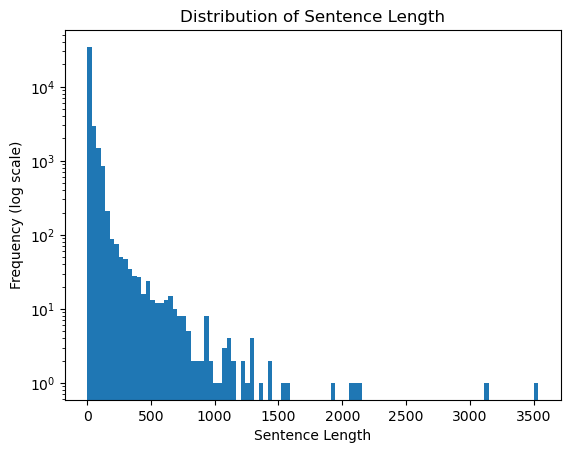
\includegraphics[width=0.8\linewidth]{Figure_sentence_length.png}
    \caption{Frequency of sentence length in the final combined dataset}
    \label[type]{sentence_fig}
\end{figure}

As an initial data processing step, we first concatenated those datasets together in order to use them to implement an initial sarcasm detection model. The final combined dataset then has the full sentence or review and a sarcastic indicator (0 or 1). The final combined dataset contains 40,461 samples from different sources and types. We then have a quite complex dataset with sentences of very variable length as displayed in figure \ref*{sentence_fig}.

\subsection{Amazon reviews dataset}

In order to explore more in depth our problematic around e-commerce, the sarcasm Amazon reviews dataset remains the most useful one in the scope of our project.
As described previously, it contains reviews of products on Amazon that are labelled either as sarcastic or regular. 
Additionally, this dataset reports other information associated to the review such as the product associated with it, the number of stars assigned by the author, etc. 
One of the sampled sarcastic reviews extracted from this dataset is given in table \ref*{tab:mytable} as an example.

\begin{table}[H]
\centering
\small
\begin{tabular}{|c|p{6cm}|}
\hline
\textbf{Feature} & \textbf{Example} \\
\hline
STARS & 3.0 \\
TITLE & Great Product, Poor Packaging \\
DATE & May 14, 2009 \\
AUTHOR & Patrick J. McGovern "Procrastinating Evil Scientist"\\
PRODUCT & Uranium Ore \\
REVIEW & I purchased this product 4.47 Billion Years ago and when I opened it today, it was half empty. \\
\hline

\end{tabular}
\caption{Example of an ironic review sample and the associated information}
\label{tab:mytable}
\end{table}

The additional information offered by this dataset will allow us to take additional parameters into account rather than basing our prediction solely on the review.
We consider that adding these features may help the model to better identify the underlying patterns of sarcasm.






%-------------------------------------------------------------------------
\section{Models}
\subsection{Simple Sarcasm detection model}
As introduced above, we build a heterogeneous dataset with sarcasm examples from very different sources and context.
Our goal here is to experiment building a model that could learn the inner structure of sarcasm from a large amount of data.

Before doing so, and as a starting point for this project, we first aimed at creating a very simple model capable of detecting if a sentence contains some from of sarcasm using the Amazon review dataset only.
At this stage, the model only takes into account the sentence and no additional factors. We will later add additional relevant factors in detecting sarcastic or humorous patterns such as information on the product considered.

Jain et al. previously conducted an experiment on this dataset~\cite{jain2019}.
Their idea was to build a feature vector for each Amazon review using various features such as the positive/negative sentiment score, punctuation, part of speech and bigram analysis.
Their results shown very good accuracy with Naïve Bayes (77.50\%), a multi-layer perceptron classifier (81\%), and SVM (81.5\%), with similar precision, recall and f1.
To verify the necessity of this feature selection, we created 2 models, one SVM and one LSTM and train them on plain data, without feature selection.
SVM used count vectorization and the LSTM used word embedding.
Our results showed that SVM performed well with 82\% accuracy on the Amazon review dataset.
However, digging into the results revealed that the model was more likely to misclassify a sarcasm text with both precision and recall being much under the ones for Regular text.
One explanation for this difference may be the small size of the dataset which contains only 1254 texts, with only 437 being sarcastic.

\begin{table}[H]
    \centering
    \begin{tabularx}{\linewidth}{|X|X|X|X|}
        \hline
        & Precision & Recall & F1-score \\
        \hline
        Regular & 0.84 & 0.90 & 0.87 \\
        \hline
        Sarcasm & 0.72 & 0.61 & 0.66 \\
        \hline
    \end{tabularx}
    \caption{Precision, Recall and F1-score for SVM on the Amazon review dataset with only count vectorization.}
\end{table}

The LSTM model on its side less performed with a test accuracy of 67\%.
A Similar behavior can be observed regarding the sarcastic text for which the model fails to understand the sarcasm pattern in all the cases.

\begin{table}[H]
    \centering
    \begin{tabularx}{\linewidth}{|X|X|X|X|}
        \hline
        & Precision & Recall & F1-score \\
        \hline
        Regular & 0.81 & 0.71 & 0.76 \\
        \hline
        Sarcasm & 0.43 & 0.57 & 0.49 \\
        \hline
    \end{tabularx}
    \caption{Precision, Recall and F1-score for LSTM on the Amazon review dataset with only count vectorization.}
\end{table}

These results confirmed the necessity of building features before training the model.

\subsection{Feature-oriented model}

Our previous experiment revealed that simple models such as SVM and LSTM do not manage to reveal the underlying structure of humorous reviews, with non-satisfactory precision and recall score on the sarcastic label.
Additionally, even though SVM performed relatively well on the test set in terms of accuracy, it may not be robust to other real word data as it is based on a Bag of Word assumption. Out of Vocabulary (OOV) tokens are very likely to occur on very diverse Amazon product review.
Thus, based on the previous research work of Jain et al~\cite{jain2019}, we implemented a new SVM model with feature selection.

The main idea of this model is to build a feature vector for each review, given metrics/criteria that are likely to reveal the sarcastic aspect of a review.
Our model uses 7 main features described bellow.

\subsubsection{Sentiment score feature}

Previous research on sarcasm classification showed that analyzing the sentiment of a review allows to give the model a first insight of the text's structure.
In our experiment, we used VADER, a lexicon and rule-based sentiment analysis tool, trained on social media content~\cite{icwsm2014}.
Amazon may not be a social media, but our intuition is that the review written by its consumers present similar structures as the texts found on social media such as X or Facebook.

One key aspect of VADER is its sensitivity to both polarity and intensity of the sentiments expressed in the text.
It also processes punctuation tokens that are used to reinforce the sentiment of a sentence.
VADER produces 4 scores for each analysis: positive, negative, neutral and compound.
The first 3 scores are ratios for proportions of text that fall in each category. The compound score is a normalized combination of the other 3.
It can be interpreted as follows:

\begin{itemize}
    \item positive sentiment: compound score $>$= 0.05
    \item neutral sentiment: (compound score $>$ -0.05) and (compound score $<$ 0.05)
    \item negative sentiment: compound score =$<$ -0.05
\end{itemize}

We used the compound score as the first feature of our model.

\subsubsection{Punctuation feature}

Sarcastic reviews are more likely to contain more exclamatory or interrogative sentences than regular texts.
Therefore, we calculate a ratio of punctuation counts over the total number of punctuation symbols in the text.

For each review, we count the following symbols: '.', '!', '?', ',' and normalize the count as explained above.
We thus produce a vector of 4 normalized counts.

\subsubsection{Part of Speech (POS) feature}

Another great indicator of potential sarcastic review is its proportion of certain grammatical tags.
This feature has demonstrated in previous studies~\cite{jain2019} its ability to reveal the humorous tone of a text.
We thus implement this feature which produce 4 normalized count of nouns, verbs, adjectives and adverbs by using the Stanza library for constituency parsing.

\subsubsection{Unigram and bigram count}

A simple intuition of how to detect sarcastic reviews is to count words that may be considered as sarcastic.
This Naïve Bayes assumption is especially relevant when using bigrams which may reveal common sarcastic word association.

To implement this feature, we build a vocabulary of sarcastic and regular unigram/bigram using the training data of the Amazon dataset.
Another approach may  be to use the vocabulary of larger dataset (such as the one we built by aggregating very diverse content), but this option was not explored during our project.

Then, for each review, we produce the ratio of unigram/bigram of the text that appear in sarcastic and regular vocabulary.

\subsubsection{Contextual feature}

This feature may be the most important/relevant for the model.
The contextual feature uses the amount of stars given by the customer in its review and compare it to the sentiment score of its review.

Indeed, one common sarcastic structure is to express the opposite of what we really think.
Thus, sarcastic reviews tend to have a strong difference between these two scores.

The contextual feature is therefore the subtraction of the normalized sentiment score (normalized on a 0 to 5 scale) and the amount of stars associated with the review.

\subsubsection{Similarity feature}

The last feature we explored is the similarity feature which is a measure of the similarity between the product title and the review given by the customer.
Our intuition was that users writing sarcastic reviews tend to use more sentences/words that are off-topic compared to the product itself.
Unfortunately, the Amazon dataset does not provide categories or other insight about the nature of the product associated with the review.

Thus, our solution consists of 3 steps:
\begin{itemize}
    \item Extract the keywords from both the title and the review. We used for this the Rapid Automatic Keyword Extraction (RAKE) algorithm which uses a combination of n-grams and stop words to extract the most relevant keywords of a text.~\cite{rake2010}
    \item For the review keywords, sort them by frequency and only keep the same amount as the amount of keywords extracted from the Title.
    \item Calculate the average similarity between the title and the review keywords using the Spacy library similarity score function. We used the 'en\_core\_web\_lg' pipeline for the similarity calculation, which is trained on written texts from online blogs, news and comments (around 560MB of data).
\end{itemize}

We thus used this average similarity score as an input feature for our model.
Data exploration revealed that the sarcastic reviews on the Amazon dataset have a global average similarity score of 0.146 with the product title associated, whereas this score is 0.157 for the regular reviews using our method.
This difference confirmed our intuition and the relevance of this feature.

\subsubsection{Training the improved SVM model}

For each review, we built a feature vector with all the above-mentioned features and the addition of the stars amount given by the user as a raw feature.
Thus, each review was represented by 16 float numbers.
We then trained an SVM model (linear kernel and default parameters of the sklearn library) on our training data and evaluate it on our validation and test sets (consisting in 125 and 126 reviews).

The results are the following for the test set:

\begin{table}[H]
    \centering
    \begin{tabularx}{\linewidth}{|X|X|X|X|}
        \hline
        & Precision & Recall & F1-score \\
        \hline
        Regular & 0.89 & 0.88 & 0.88 \\
        \hline
        Sarcasm & 0.70 & 0.72 & 0.71 \\
        \hline
    \end{tabularx}
    \caption{Precision, Recall and F1-score for SVM on the Amazon review dataset using feature selection}
\end{table}

Compared to our previous SVM model, we can observe that the recall of the sarcasm label is much improved by 10\%.
Overall, our model is more stable and less sensitive to new data.
The accuracy measured is 0.86 on the validation set and 0.83 on the test set.

This experiment demonstrates that a simple model like SVM manage to understand the structure of sarcasm when using the appropriate features.
Training a fully connected deep neural network on these features may produce better results, but we did not have the time to explore this path.

Next, we train a state-of the art transformer model to observe if it can generalize sarcasm on our combined and general dataset.

\subsection{BERT-based Sarcasm Detection Model}
\subsubsection{Overview of BERT}
Bidirectional Encoder Representations from Transformers (BERT) was a significant advancement in the field of natural language processing (NLP), as it leverages the Transformer, a state-of-the-art neural network architecture specifically built to effectively process sequential input.
In contrast to conventional models that operate on text unidirectionally (either left-to-right or right-to-left), BERT stands out due to its capacity to comprehend the contextual meaning of a word within a sentence by considering the preceding and succeeding words, thus enabling bidirectional processing of the entire word sequence.
The aforementioned feature is especially beneficial in tasks such as sarcasm identification, where the contextual interpretation of words plays a crucial role in determining the presence of sarcasm in a statement.

\subsubsection{Model Implementation}
In our sarcasm detection task, we utilized a pre-trained BERT model, which we then fine-tuned on a dataset consisting of texts labeled as sarcastic or non-sarcastic. 
By fine-tuning BERT on our specific dataset, the model could apply its deep, bidirectional understanding of language to effectively distinguish between sarcastic and genuine statements.

\subsubsection{Experimental Results}
The efficiency of our fine-tuned BERT model in sarcasm detection was significant. 
The validation loss obtained was 0.386, while the accuracy reached was 87.823\% on the test set sampled from our 40,461 text dataset introduced previously. 
The findings of this study emphasize the proficiency of BERT in effectively categorizing sentences as either sarcastic or non-sarcastic, hence showcasing its sophisticated comprehension of language and contextual nuances.

\subsubsection{Conclusions}
The efficacy of our BERT-derived model in detecting sarcasm illustrates the robustness of bidirectional contextual analysis in comprehending intricate linguistic patterns. 
The experimental results demonstrate that BERT is effective in handling delicate natural language processing (NLP) tasks, specifically sarcasm detection, as seen by its high accuracy and minimal validation loss.
The aforementioned efficacy highlights the wider possibilities of employing advanced, contextually-aware models in complex language comprehension tasks.


\subsection{Sarcasm detection with additional factors}

\subsection{ColBERT Sarcasm Detection Model}
Contextualized Late Interaction over BERT is a novel ranking model that adapts BERT for efficient retrieval.
Traditionally, BERT models can be computationally expensive and memory-intensive.

Those particularities make it challenging to apply for some tasks such as passage retrieval in search engines.
In the scope of our project, such a model can be useful in our task of sarcasm detection.

The key idea behind ColBERT is to use a late interaction mechanism between different tokens of the original sample.
The proposal of this model is based on the observation that usually a joke can involve two or three stages of storytelling that are sometimes concluded with a punchline.
Theories state that humor arises from the sudden transformation of an expectation into nothing.
The punchline is, in that sense, related to the previous sentences, but often creates an opposition in order to transform a reader's expectation of the context.
With that being said, if one reads the sentences of a joke separately, they are likely not going to be found funny.
However, if those same sentences are read together, the text becomes humorous.
This is why a model that extracts features independently from each sentence and then considers those features later can be interesting in sarcasm detection.

We propose here to separate sentences from a sample and use the BERT model to create embeddings for each sentence.
The embeddings are then passed through separate hidden layers to extract each feature. Finally, the results are concatenated and passed through a neural network to predict the target value.

An additional preprocessing step is necessary in order to remove from the dataset samples that are too long.

\begin{figure}[H]
    \centering
    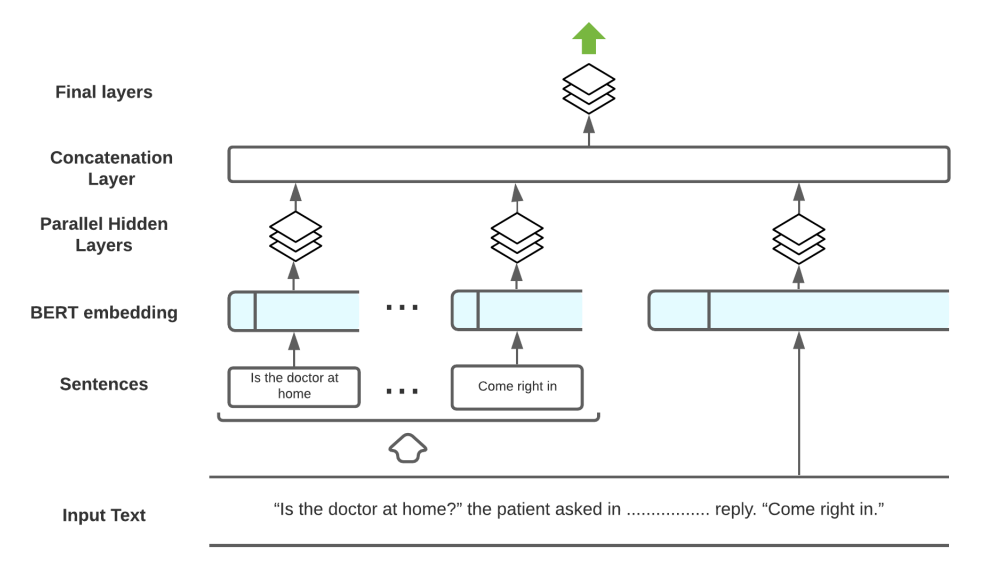
\includegraphics[width=0.9\linewidth]{ColBERT_model.png}
    \caption{Architecture of the ColBERT model}
    \label[type]{sentence_fig}
\end{figure}

An architecture of the ColBERT model is given above. In addition to the sentences processed individually, it remains important to detect word interactions in the whole text.
This is why we will also feed the whole text in its own parallel line and concatenate the results with features extracted from the other networks.


Results in the literature have shown that ColBERT performs in fact quite well in sarcasm detection. It would have been interesting to check if such a model performed better than our BERT model presented previously.
Unfortunately, our attempts at coding this model were inconclusive, but we believe that splitting the text as such into sentences processed independently is key to improving sarcasm detection.


\subsection{Comparison with Chat-GPT}
In order to enhance the depth of our analysis, we conducted a comparative evaluation between our sarcasm detection model and Chat-GPT, primarily focusing on the GPT-3.5-turbo variant developed by OpenAI.
The objective of this comparison was to assess the efficacy of our model in comparison to a widely recognized general-purpose language model.

\subsubsection{Methodology}
Our approach involved querying Chat-GPT with a set of sentences from our dataset, asking it to determine if each was sarcastic.
The queries were formulated in a simple way, while we recognize that the design of the prompt was not extensively optimized and may need more modification to improve accuracy.
This observation suggests the possibility of making enhancements in further experimental endeavors.

\subsubsection{Observations \& Thoughts}
The preliminary results of Chat-GPT on our sarcasm detection test were unsatisfactory, exhibiting an accuracy rate of merely 59.75\%.
The actual application of Chat-GPT was hindered by the time-consuming nature of its interaction, mostly caused by the response latency and rate limiting of the API. This limitation had a notable impact on the usability of Chat-GPT in many circumstances.
Furthermore, the responses generated by Chat-GPT occasionally deviated from the intended aim, most likely related to its broad training and reliance on the provided prompts.

Moreover, the financial aspect associated with the utilization of GPT-3.5-turbo proved to be significant, especially considering its rather limited precision as observed in our conducted evaluations.
Taking into account these factors, including the processing requirements and concerns regarding response time, raises doubts about the viability of utilizing this approach for sarcasm detection in e-commerce environments on a big scale or in real-time scenarios.
Subsequent examinations may be conducted to assess the potentialities of GPT-4; nevertheless, the substantial cost associated with its utilization constitutes a pivotal aspect requiring careful deliberation.

%-------------------------------------------------------------------------

\section{Conclusion}

Our project aimed to explore various potential solutions to unmask sarcasm in e-commerce reviews.
Our goal was to determine which models can be use for this specific task, and their trade-off regarding cost and complexity.
We observed that simple models, such as SVM, can be very efficient to unmask sarcasm in the vast majority of reviews, when paired with relevant features extraction over the data.
However, sarcasm being a complex human mechanism, some humorous reviews are much more complex to identify, especially when the 'joke' is conducted over a long text.
To this extent, state-of-the-art transformer models have proven to be extremely effective, with our BERT model reaching a precision of 99\% on classifying non-humorous review, and 91\% for the sarcastic texts on our combined dataset.
Its only apparent weakness being the recall of sarcastic reviews falling to 75\%.
We also observed that the BERT model using transfer learning from the combined dataset did not perform better when combined with additional features from the product review such as the number of stars and the product title.
Finally, our experiment on ChatGPT highlighted that generative models using LLMs are no great sarcasm classifier, confirming our initial intuition.
By doing so, we wanted to show that these models, that tend to be over-hyped and over-used, may not be an ideal solution, especially when considering their cost and slowness.

As a conclusion, our project highlighted the necessity of understanding the structure of sarcasm to choose a relevant model.
We learned a lot during this project, and it gave us great experience on a real word deep-learning problem, especially on the hard and time-consuming tasks such as fine-tuning and data preparation.

Future work on this topic may include finishing the Colbert implementation which we unfortunately did not manage to do in time.
A great application of our work may also be to use our classification model to then rephrase sarcasm review into unambiguous texts.
This could be use as an inclusive tool on e-commerce platforms, as people suffering from language or autism pathologies may struggle to understand the sarcasm tone of a review.

%-------------------------------------------------------------------------

%%%%%%%%% REFERENCES

\nocite{*}
{\small
\bibliographystyle{ieee_fullname}
\bibliography{egbib}
}

\end{document}
